\chapter{Analytical Model}
\label{ch:analyticalmodel}

\section{Foundation of the quasiclassical model}
\begin{figure}
\centering
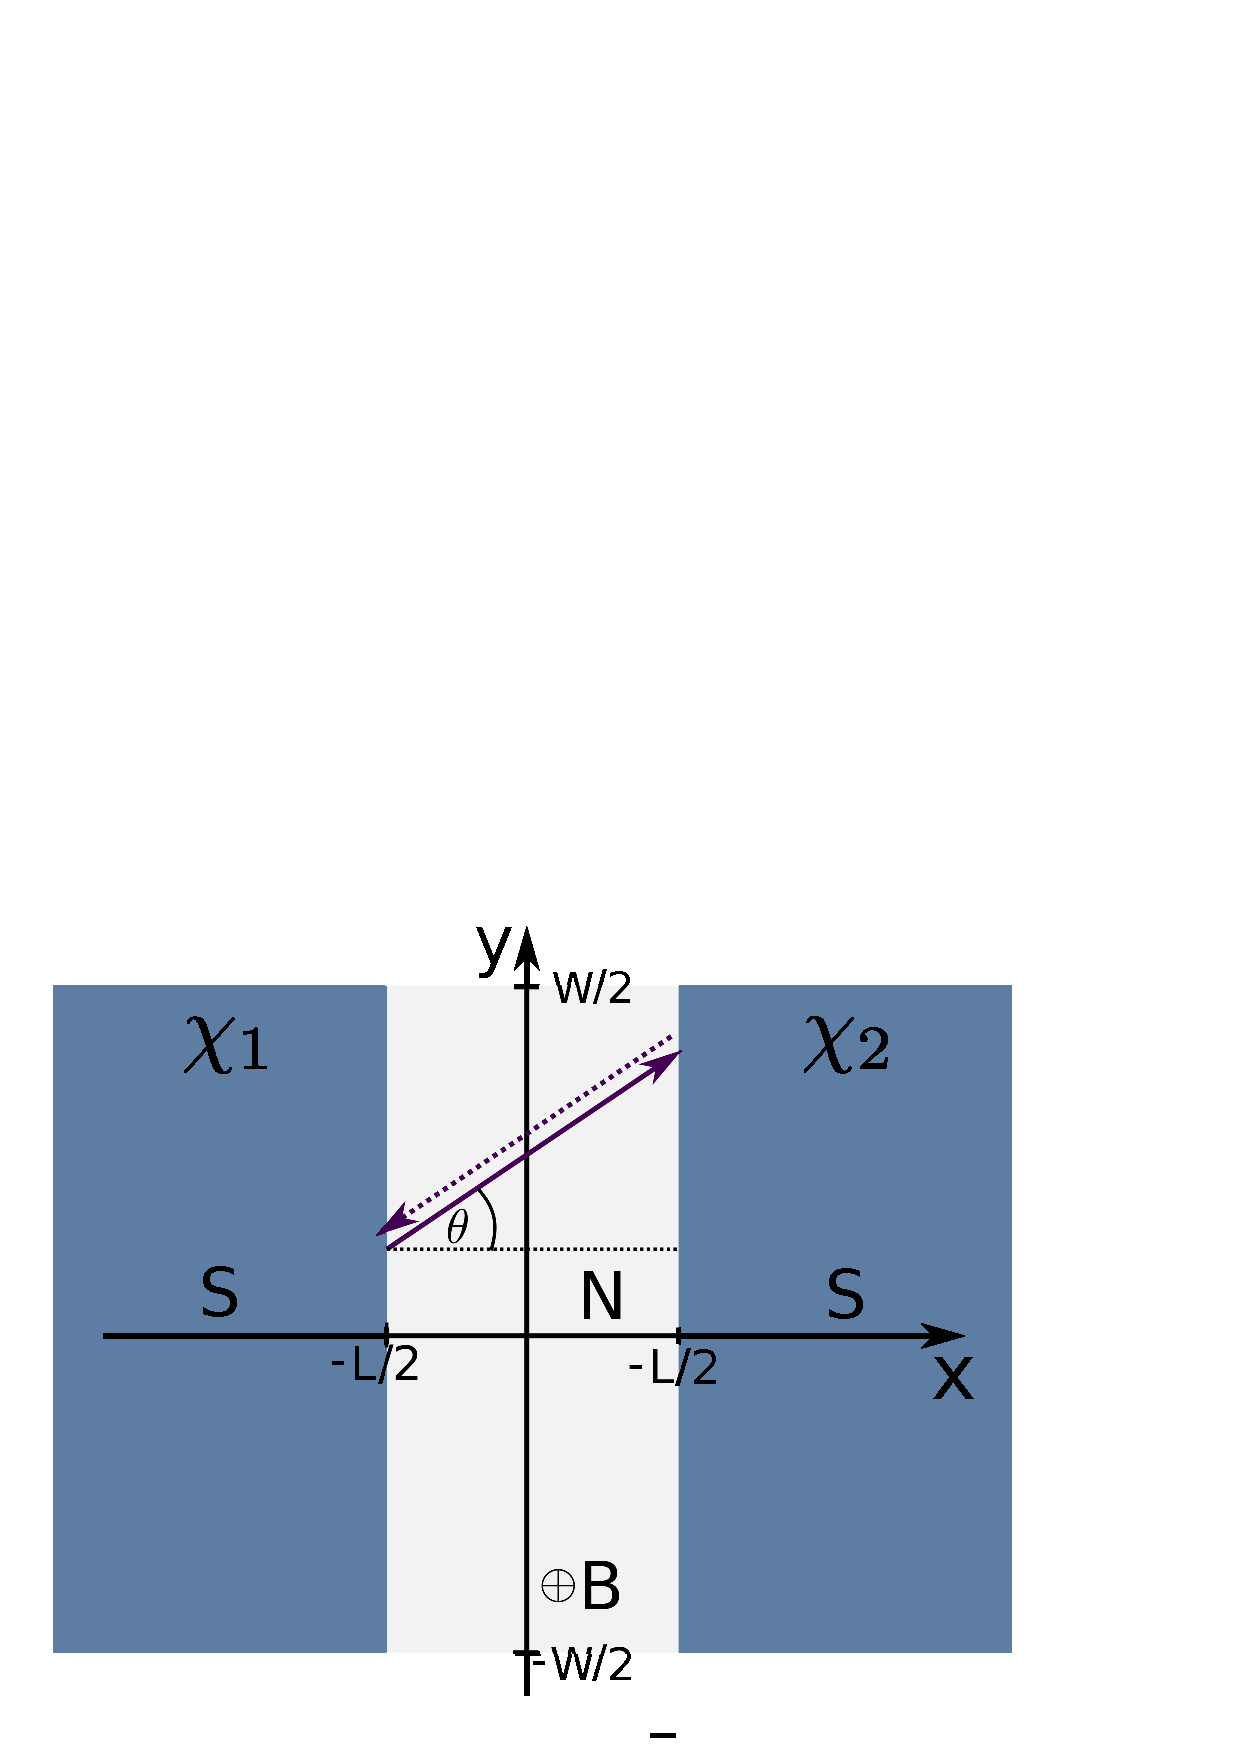
\includegraphics[width=0.6\textwidth]{figure/analyticalmodel/sns_junction.pdf}
\caption{Schematic representation of a short and wide SNS junction.}
\label{fig:sns_schematic}
\end{figure}

In figure \ref{fig:sns_schematic} a schematic SNS junction is depicted. The setup is two dimensional with width $W$ and length $L$. The NS-interfaces are parallel to the $y$-axis and are placed at $x = \pm L/2$. Each of the superconducting leads has a phase $\chi_{1}$ and $\chi_{2}$ and the overall phase difference is $\chi = \chi_{1} - \chi_{2}$. The superconducting gap parameter is only present in the superconducting leads and zero in the normal region and can be expressed as
\begin{equation}
\Delta\left( x \right) = |\Delta| e^{\chi_1} \Theta\left(-L/2 -x \right) + |\Delta| e^{\chi_2} \Theta\left(x-L/2 \right) 
\label{eq:gap_parameter}
\end{equation}
The aim is to express the current through the junction using a quasiclassical approach. In this approach, the Andreev bound states are assosiated with straight trajectories connecting the superconducting leads. The superconducting current density is expressed in terms of these trajectories. We consider a ballistic sample with ballistic (BCS) coherence length $\zeta = \hbar v_F / \pi \Delta$ %TODO check!
We assume that at this coherence length $\zeta$ is much larger than the Fermi velocity $\zeta \gg v_F$ (in order to induce superconductivity in the system?). The relation between the coherence length $\zeta$ and the sample length $L$ determines, if the considered junction is a \textit{short} or a \textit{long} junction:
\begin{eqnarray*}
\zeta \ll L \quad \rightarrow \quad \text{long junction} \quad \rightarrow \quad \text{many Andreev levels} \\ 
\zeta \gg L \quad \rightarrow \quad \text{short junction} \quad \rightarrow \quad \text{one Andreev level} 
\end{eqnarray*}
Needless to mention, the fermi wavelength $\lambda_F$ has to be smaller than the sample length $L$. 
Now, check if this quasiclassical approach is valid. What are preliminary assumptions about the system?
%TODO klar machen, dass jetzt die Voraussetzungen für Modell getestet werden
The presence of magnetic field will lead to a bending of the trajectories due to the Lorentz force. Depending on the strength of magnetic field $B$ and the Fermi velocity the radius of this curve is 
\begin{equation}
r_B = ???
\end{equation}
%TODO add the formula for cyclotron radius
In order to justify the assumption of straight trajectories, either the magnetic field has to be weak enough or the Fermi wavelength has to be short enough. Then, the cyclotron radius $r_B$ is simply much smaller than the sample length $L$. 
We consider the low temperature limit, where the thermal length scale of the system is smaller larger than the sample length:
\begin{equation}
L_T = \hbar v_F / k_B T \gg L
\end{equation} 
%TODO what do these length scales mean? Add!

\section{Plane setup: calculation of current}
%TODO Re-calculate current from Glazman
To derive the current for the SNS setup depicted in figure \ref{fig:sns_schematic}, we start by writing down the Bogoliubov-de-Gennes-Hamiltonian for this system.
\begin{equation}
\begin{pmatrix}
-\frac{1}{2m} \nabla^2 - \epsilon_F & \Delta(x) \\
\Delta^*(x) & \frac{1}{2m} \nabla^2 + \epsilon_F 
\end{pmatrix}
\begin{pmatrix}
\psi_e \\
\psi_h
\end{pmatrix} = E 
\begin{pmatrix}
\psi_e\\
\psi_h
\end{pmatrix}
\end{equation}
This expression uses eq. (\ref{eq:gap_parameter}) for the spatially dependent superconducting gap parameter $\Delta(x)$.

This Schrödinger equation can be solved with boundary conditions at $x = \pm L/2$ and leads to the following wave functions
\section{QPC setup: calculation of current}
\begin{figure}
\centering
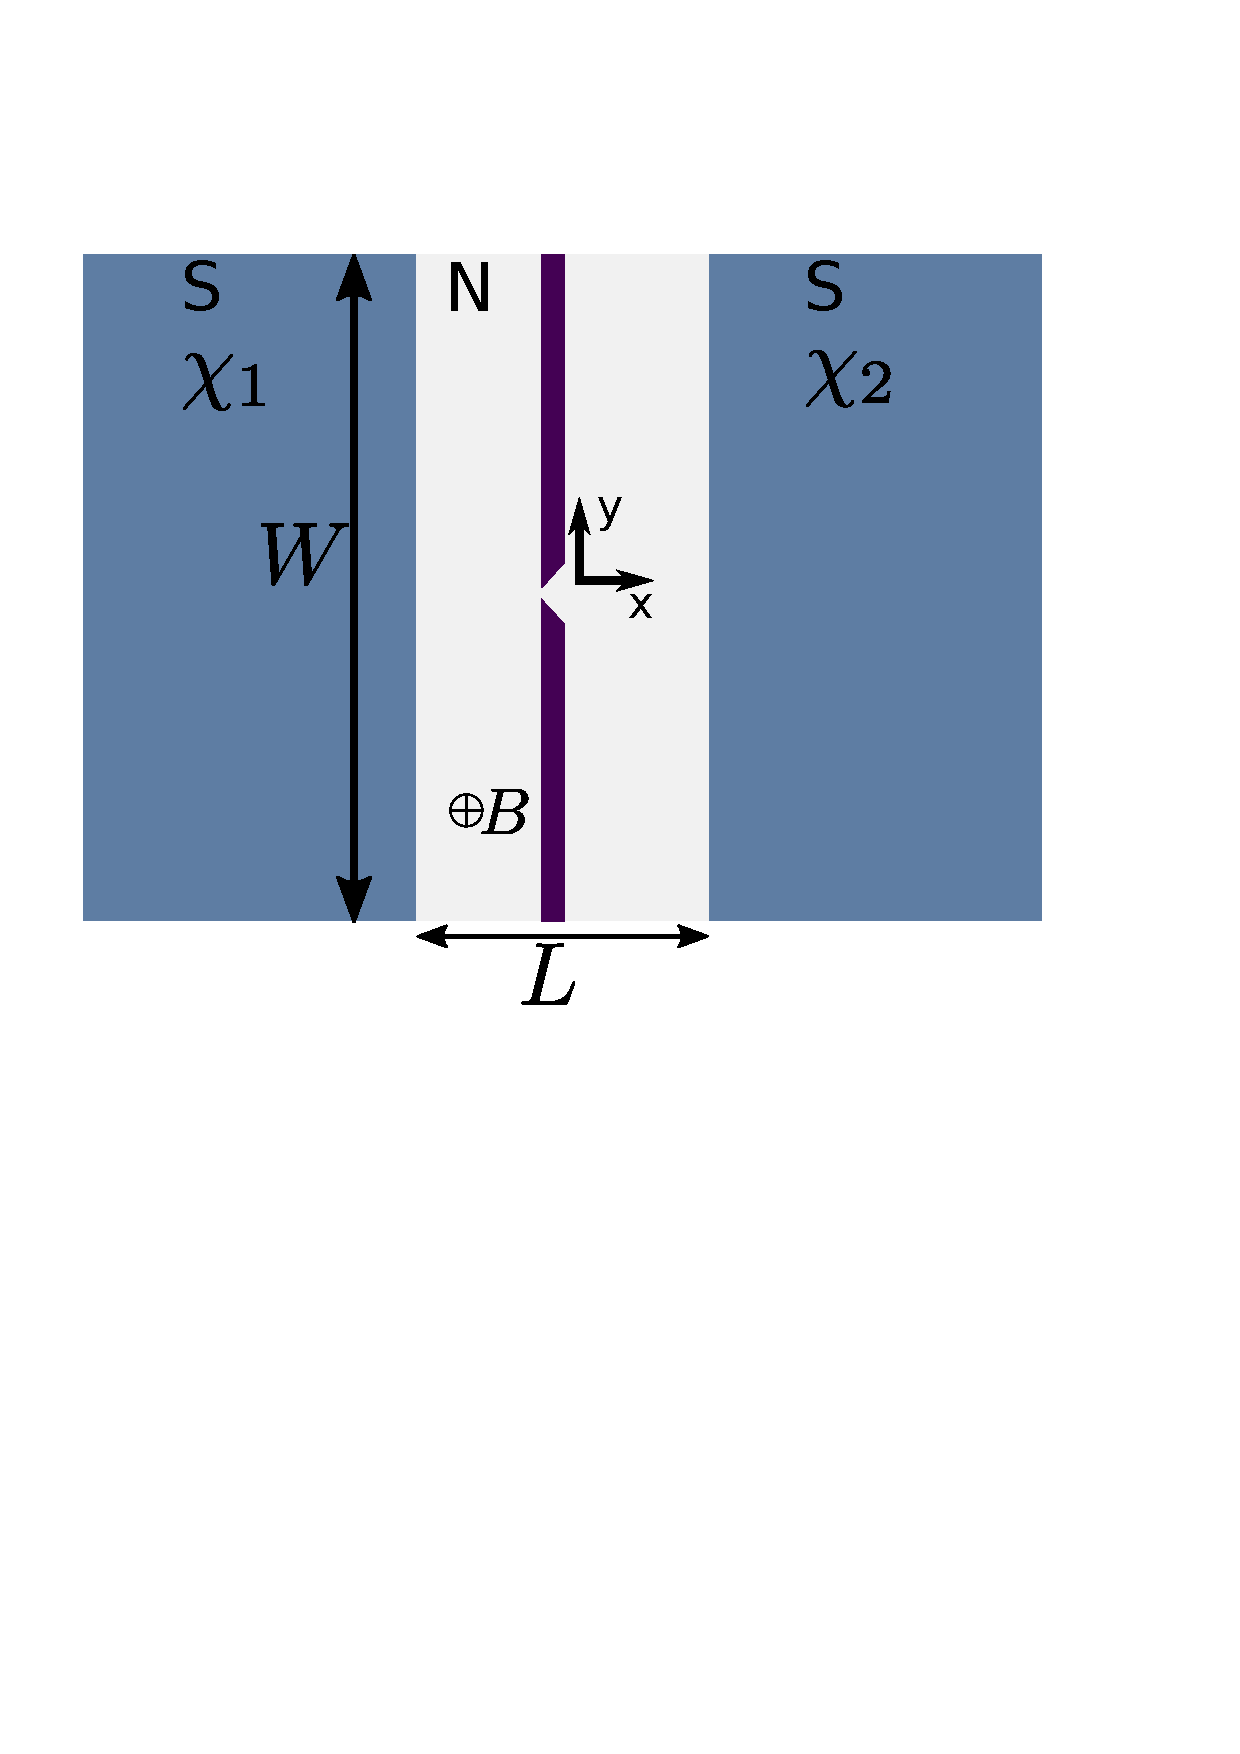
\includegraphics[width=0.6\textwidth]{figure/analyticalmodel/qpc_sns_junction.pdf}
\caption{Schematic representation of a short and wide SNS junction with QPC setup.}
\label{fig:qpc_sns_schematic}
\end{figure}

